\documentclass[plain,basic]{inVerba-notes}

\newcommand{\userName}{Cullyn Newman}
\newcommand{\class}{BI:\@ 428}
\newcommand{\theTitle}{Journal Article Summary --- Week 8}
\newcommand{\institution}{Portland State University}
%chktex-file 8
\begin{document}    

\begin{center}
    \textbf{\LARGE{Conformation of sister chromatids in the 
    replicated human genome}}
\end{center}

\section{Background}
\begin{itemize}
    \item \textbf{Chromosome conformation capture}: a set of molecular biology methods used to analyze the spatial organization of chromatin in a cell. 
        \begin{itemize}
            \item Done by quantifying the number of interactions between genomic loci that are nearby in space. These interactions are often actually separated by many nucleotides, which makes understanding interactions hard when looking at the genome linearly. 
            \item There are various types of methods used to quantify the interactions, but this paper uses a specialized method of chromosome conformation capture.
        \end{itemize}
    \end{itemize}

    \begin{center}
        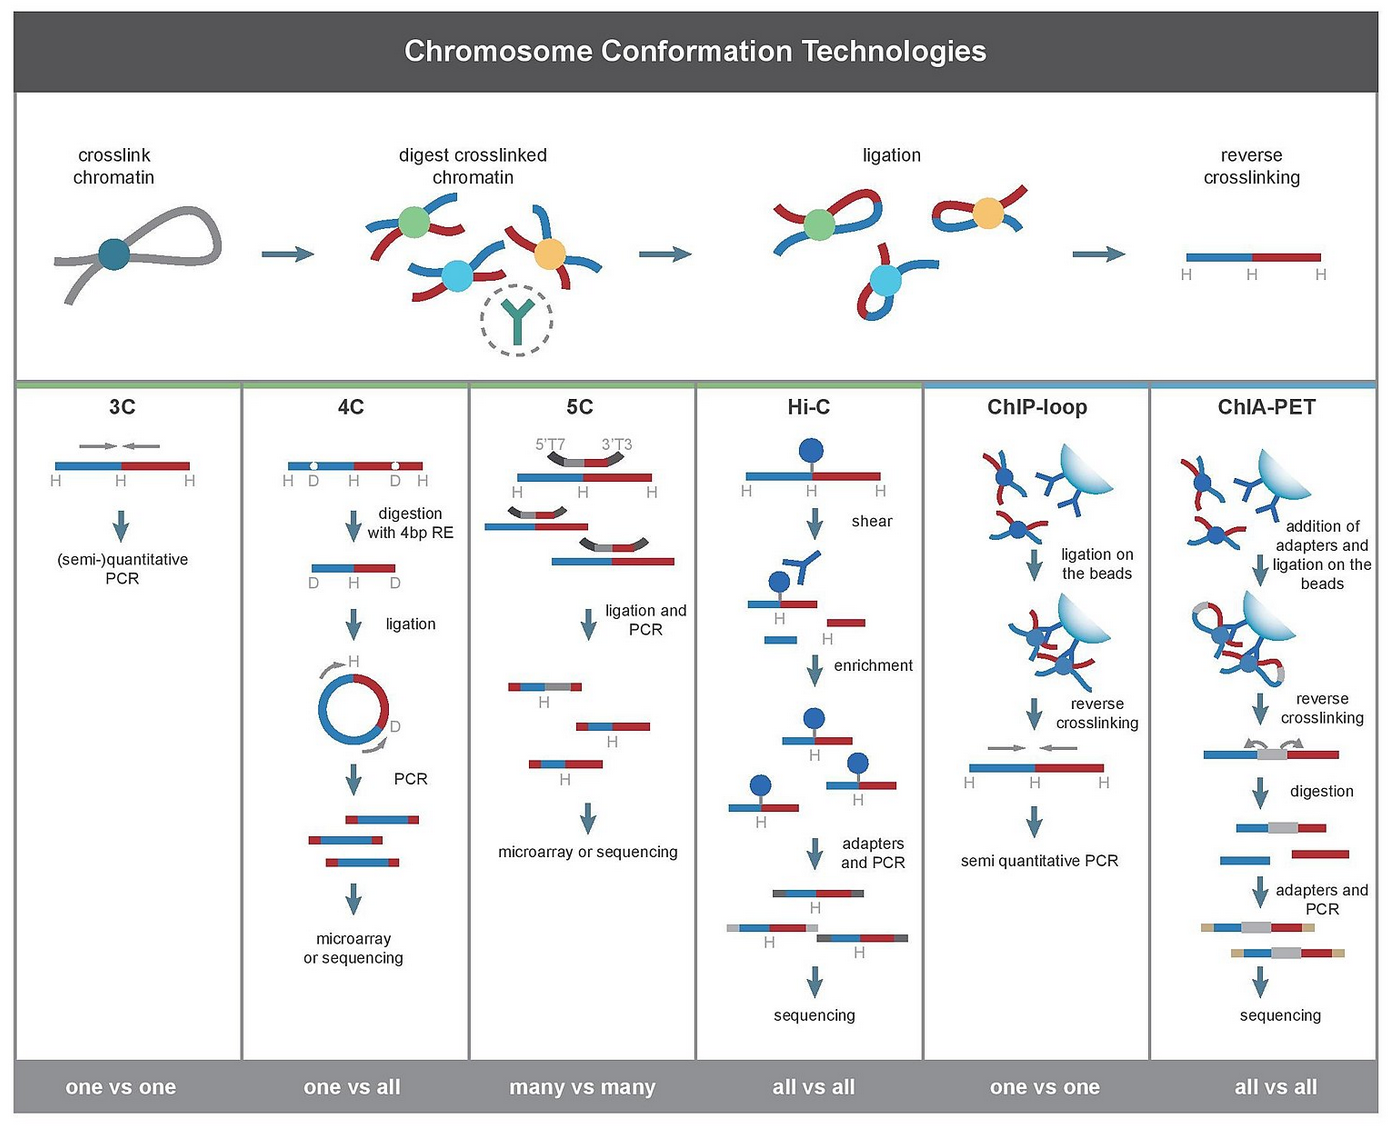
\includegraphics[scale=0.32]{images/8-3c.png}
    \end{center}
    
    \begin{itemize}
    \item \textbf{Hi-C (all-vs-all)}: a method of chromosome conformation capture that uses high-throughput sequencing to find the nucleotide sequence of fragments by using paired end sequencing (shotgun sequencing), which retrieves a short sequence from each end of a ligated fragment. 
        \begin{itemize}
            \item Generally, H-C allows for two sequences that should represent different restriction fragments to be ligated together in the proximity based ligation step.
            \item The pairs of sequences are then individually aligned to the genome, allowing for the determination of fragments involved in the ligation event. This allows for all possible pairwise interactions between fragments to be tested.
        \end{itemize}
    \item \textbf{Topologically associating domain (TAD)}: a self-interacting genomic region, where particular DNA sequences physically interact with each other more frequently than sequences outside the TAD\@. These regions often influence gene expression via interactions with enhancer-promotor interactions.
        \begin{itemize}
            \item Boundaries at both sides of the TADs are often conserved between mammalian cell types, with highly enriched CCCTC-binding factor (CTCF) and cohesin (a protein complex that mediates several functions, including DNA looping in TADs). 
            \item Influence over these TADs allow for various chromosomal organization and conformation changes, leading to contributions to regulation of transcription, development disorders, cancer, and DNA repair.
            \item However, it's not known how cohesive linkages distribute on the genome to support these functions, and how they are coordinated with dynamic loop formation in TADs.
        \end{itemize}
    \item Normal Hi-C technology cannot be used to explore topological interactions between sister chromatids of replicated chromosomes, since the identical DNA sequences in replicated chromosomes makes it impossible to distinguish between intramolecular and intermolecular contacts. This was obstacle that authors of this paper aimed to overcome by creating a specialized Hi-C method. 
\end{itemize}

\section{Sister-chromatid-sensitive Hi-C}
\begin{center}
    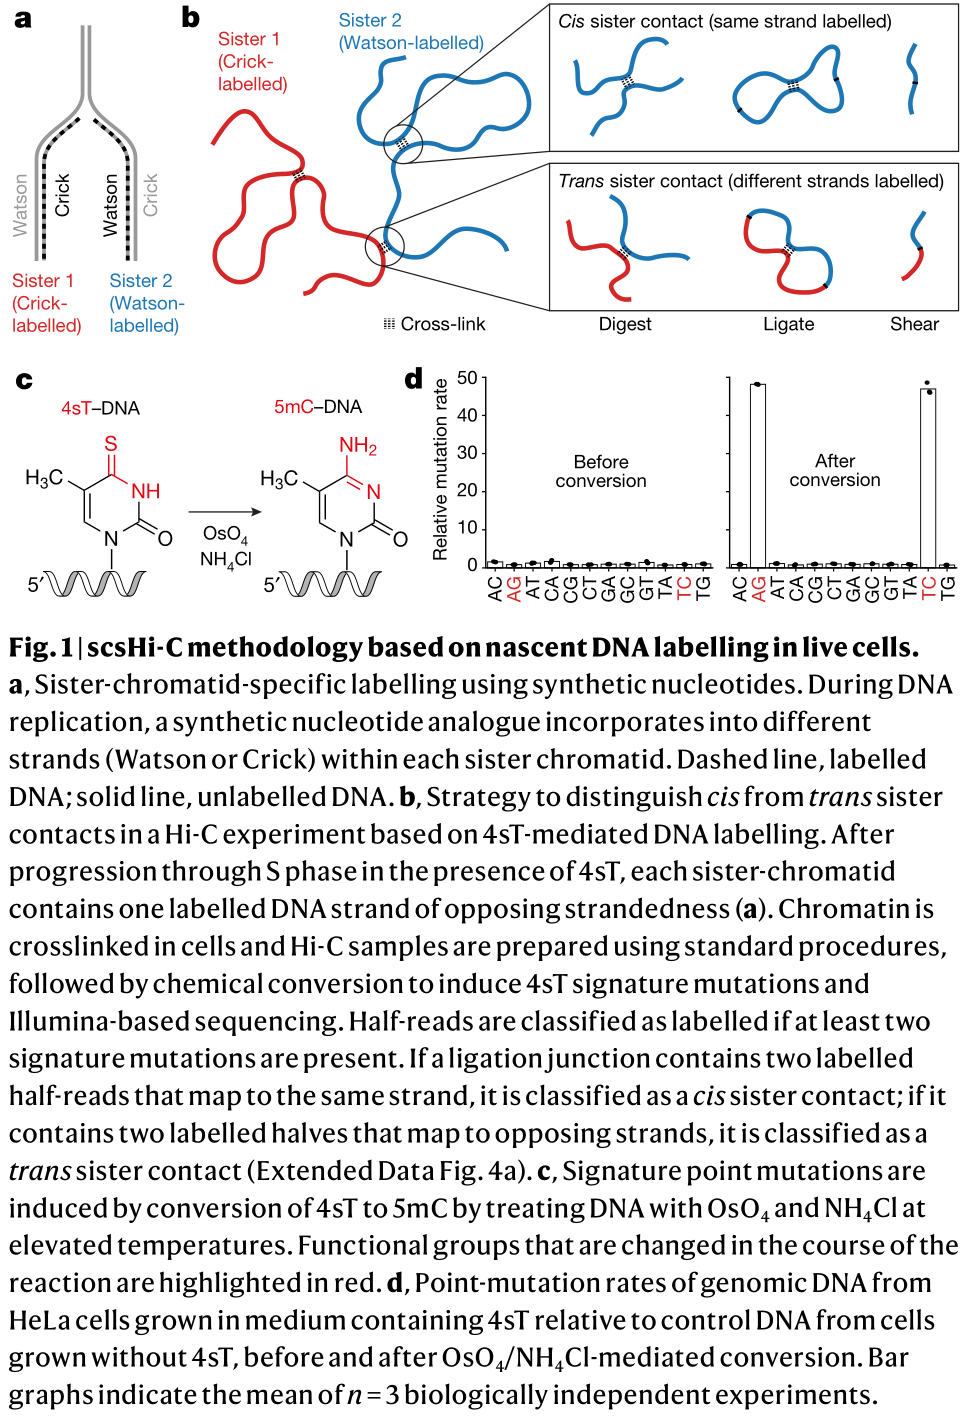
\includegraphics[scale=0.42]{images/8-1.png}
\end{center}
\begin{itemize}
    \item \textbf{Sister-chromatid-sensitive Hi-C (scsHi-C)}: specialized DNA labeling of sister-chromatids in order to distinguish between strands for Hi-C method, allowing for the genome-wide analysis of sister-chromatid interactions in human cells.
\end{itemize}

\section{Conformation of replicated chromosomes}
\begin{itemize}
    \item Using scsHi-C, the authors were able to investigate and measure the extent of sister-chromatid resolution during mitosis by constructing genome-wide scsHi-C maps of cells synchronized to G2 or mitotic prometaphse.
    \item I wasn't exactly how they were using the data generated in figure two below, but what is appeared to indicate was that TADs set the limits of discrete domains with variable degrees of sister-chromatid pairing, with the overall degree of sister-chromatid pairing within TADs defined by characteristic chromatin modifications.
\end{itemize}
\begin{center}
    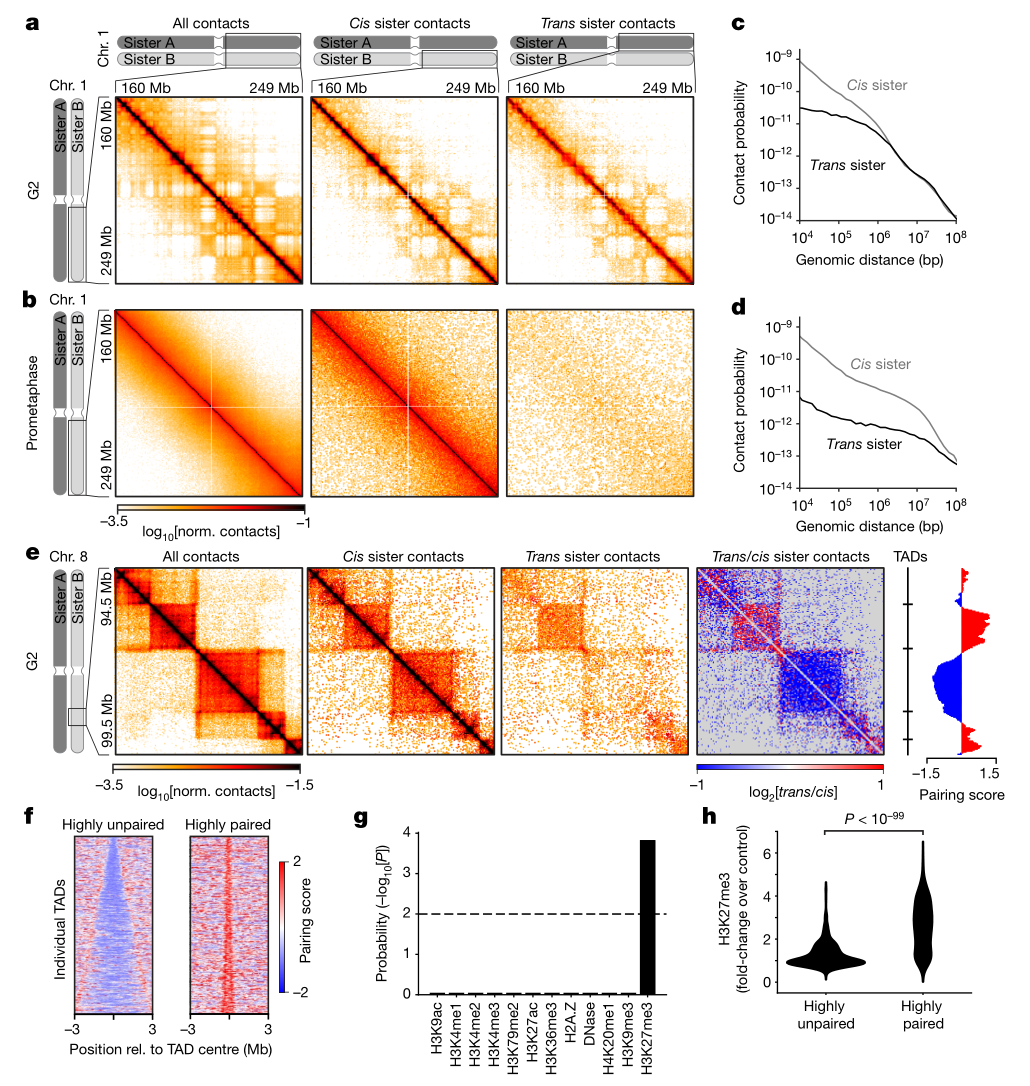
\includegraphics[scale=0.44]{images/8-2.png}
\end{center}

\newpage
\section{TADs in replicated chromosomes}
\begin{itemize}
    \item Next, the authors investigated how chromatin fibers fold within individual TADs.
    \item \textit{Cis} were mostly found along the diagonal of TADs, indicating frequent short-range intramolecular contacts.
    \item \textit{Trans} filled TAD areas without substantial accumulation along the diagonal, indicating that sister DNAs are not strictly aligned in a ``railroad'' configuration within TADs.
    \item \textit{Trans} contact maps (b) and aggregated contact probability maps of TADs (c) showed that \textit{trans} sister contacts were enriched at TAD boundaries and at corner positions connecting neighboring boundaries.
    \item Overall, sister-chromatids are predominantly liked at TAD boundaries, where they separate extensively inside TADs.
\end{itemize}
\begin{center}
    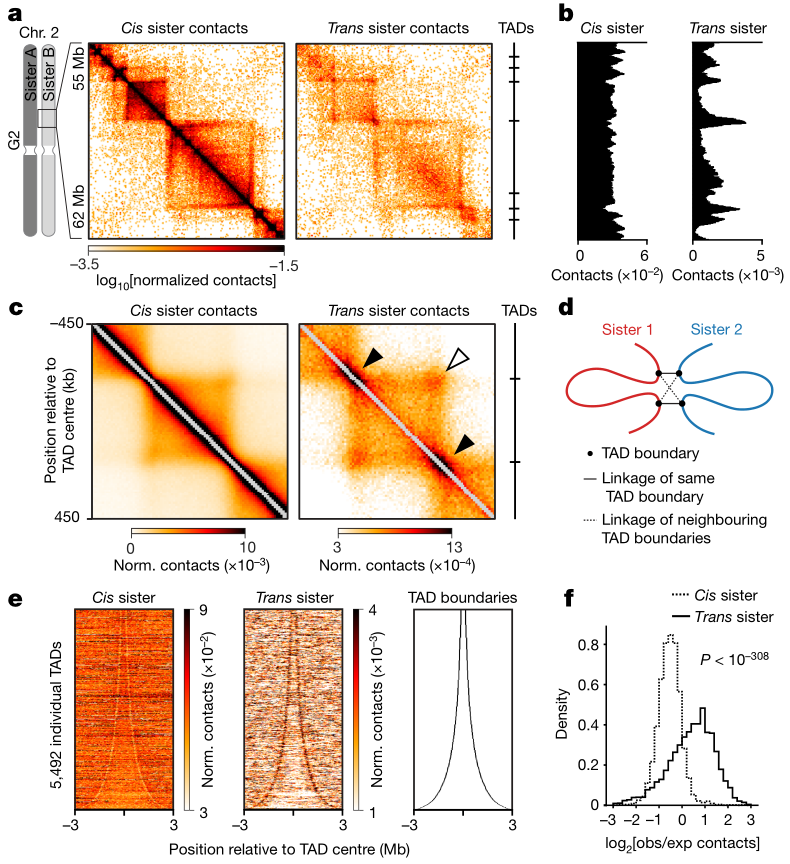
\includegraphics[scale=0.5]{images/8-3.png}
\end{center}

\section{Control of sister-chromatid topologies}
\begin{itemize}
    \item Durign G2 phase, about half of all chromatin-bound cohesin dynamically turns over to form \textit{cis}-chromatid loops that shape TADs, whereas the other half binds soroin and persistently links sister chromatids.
    \item It is possible that \textit{trans} sister contacts concentrate at TAD boundaries due to motor-driven loop extrusion, or through a mechanism that involves cohesin independently of DNA loops.
    \item Again, I'm not exactly sure how the data below was used to draw the conclusions, so I'm going to reframe from inaccurately trying to describe it. However, what they did find is that loop-forming cohesin is necessary to separate sister chromatids within TADs resulting in locally enriched sister-chromatid contacts at the boundaries, meaning that it contributes to the formation of discrete highly paired domains.
    \item Additionally, they found that the sororin-stabilized pool of cohesin is not required to form intra-chromatid loops or TADs in G2, but it is required to prevent the separation of sister chromatids and maintain their global alignment during the G2 phase.
\end{itemize}
\begin{center}
    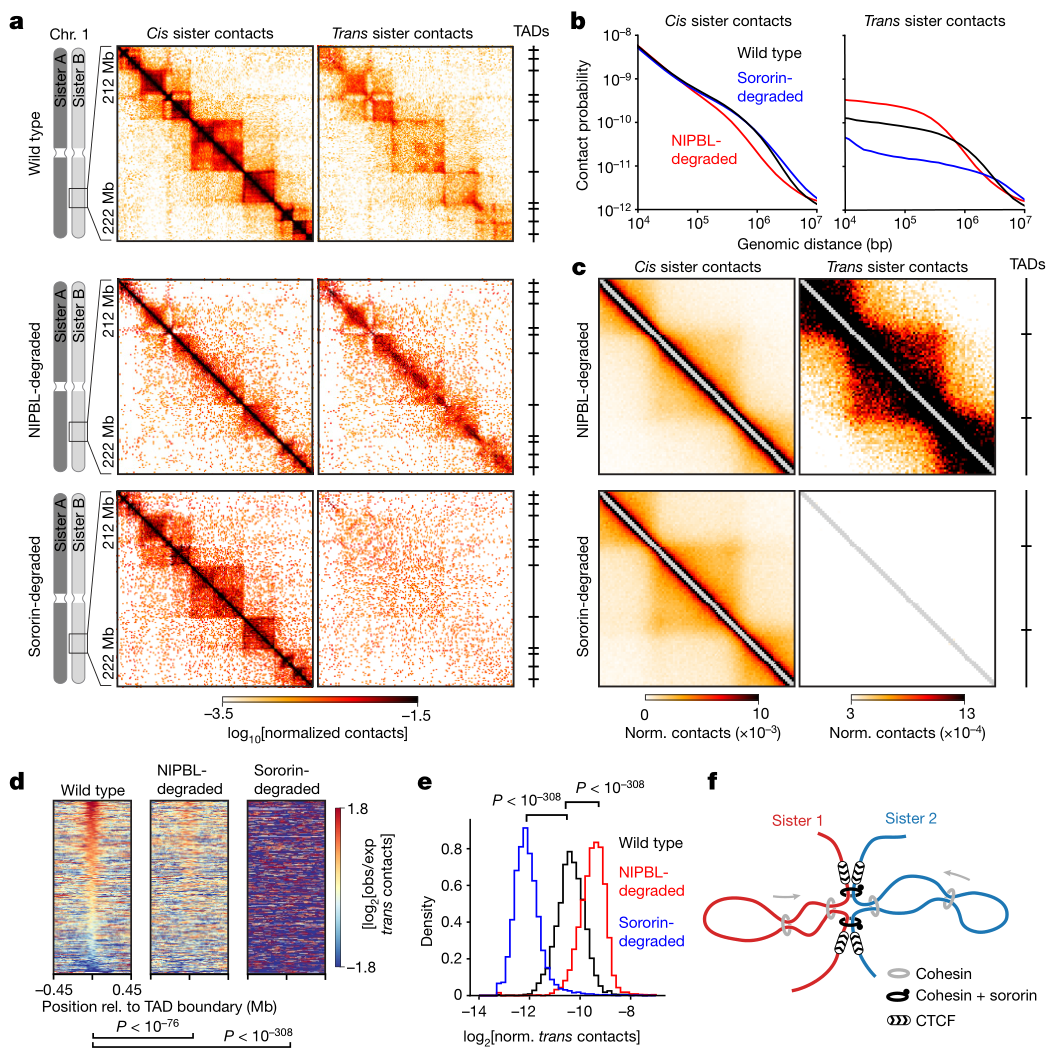
\includegraphics[scale=0.38]{images/8-4.png}
\end{center}

\section{Conclusion}
\begin{itemize}
    \item Their scsHi-C analysis showed that a pool of cohensin that mediates linkage between replicated DNA molecules maintains the alignment of sister chromatids after DNA replication.
    \item Also, another pool of cohesin that dynamically forms loops locally separates sister chromatids within TADs during G2.
    \item An independent study in a fungus reproduced similar results found in this study using the same method.
    \item The scsHi-C method allows for investigation of the organization of sister chromatids and has implications for understanding the maintenance, expression, and mechanical transport of the genome.
    \item The global alignment of sister-chromatid arms by sororin-stabilized cohesin favors interactions between homologous genome regions, as required for error-free homology-directed DNA damage repair.
    \item How the other coordinated activities that allow sister-chromatid resolution and thus allows for cells to resolve whole chromosome arms when entering mitosis remains unknown ScsHi-C may allow for the investigation of such mechanisms and others, possibly such as how pairing and recombination of homologous chromosomes occur during meiosis. 
\end{itemize}

\nocite{mitter2020conformation}
\bibliographystyle{apacite}
\bibliography{summaries.bib}
\end{document}
